\subsection{Experimental results on alternative metrics}

%To further study the relations between each of the three above metrics
%and the semantic scores, we conducted several experiments in the same
%manner as the previous study described in
%Section~\ref{sec:bleuresult}. We then present our proposed metric
%in Section~7 based on the results of the following experiments.

To evaluate the abilities of STS, TRS and GRS in reflecting the
semantic accuracy of translated code, we conducted three experiments
for these three metrics in the same manner as the study described in
Section~\ref{sec:bleuresult}.

The correlation coefficient results between each of the three metrics
with semantic score are described in
Table~\ref{table:correlation}. These results follow a similar trend:
for each model, the correlation coefficients increase constantly
according the abstraction levels of source code from text, AST, to PDG
in three metrics. For example, for mppSMT, the correlation
coefficient between STS and semantic score is 0.549, whereas that
for TRS is much greater at 0.820. The highest value is the
correlation coefficient is between GRS and semantic score at 0.910. A
reason for this phenomenon is that for a pair of source code, if they
are textually identical, they have the same AST representation, and
the exact-match in AST leads to the equivalence between the
corresponding PDGs. Meanwhile, the equivalence in a higher
abstraction level does not necessarily lead to the equivalence in a
lower abstraction. For example, Fig.~\ref{fig:mppSMT_example} shows
two methods with equivalent PDGs, but textually~different. 

Despite of the increase of the correlation coefficients, GRS and TRS
are used to measure subsets of methods in our sample set 
(table \ref{table:metrics}), and the sizes of GRS are greater than 
TRS's ones, whereas STS is able to apply for all cases. For example, 
the applicable sets of methods translated by lpSMT are quite limited, 
75 and 123 (out of 375 methods) for GRS and TRS respectively. The reason
for this phenomenon is that to construct the higher level representations,
the translated results need to satisfy certain syntactic and semantic related
constraints such as resolvable data and control dependencies.
\begin{table}
\centering
\caption{Numbers of applicable methods of metrics}
\begin{tabular}{|c|c|c|}
\hline
  & GRS & TRS\\
\hline
GNMT  & 128 & 155  \\
\hline
mppSMT  & 239 & 292 \\
\hline
lpSMT & 75 & 123 \\
\hline
\end{tabular}
\label{table:metrics}
\end{table}

Based on these empirical results, we conclude that the metric that
measures the results in the higher abstraction level, the better
metric for reflecting the semantics accuracy.  However, the higher
representation like PDG cannot always be constructed because of
missing required information in the translated results. Therefore, in
Section~\ref{sec:proposal}, we propose a metric to evaluate the
quality of translated code, that combines the measurement of the
similarity of translated code and expected results in multiple
representations.

%It is not worth to use SED instead of BLEU since it still has the same
%problems as BLEU while its advantage is insignificant.
%We then present our proposed metric in section~7 based on the results of the following experiments.

%To verify the 3 metrics SED, TREED, and GVED , we conducted an exploratory study that reveals their correlation with the ground truth Semantic score. Table \ref{table:correlation} summarizes our results for the two models mppSMT and lpSMT. We will explain each metric \rq s correlation in details as follows:

\begin{table}
\centering
\caption{Correlation coefficients with semantic score}
\begin{tabular}{|c|c|c|c|c|}
\hline
 & STS & TRS & GRS\\
\hline
mppSMT  & 0.549 & 0.820 & 0.910 \\
\hline
lpSMT  & 0.533 & 0.786 & 0.823 \\
\hline
GNMT & 0.692 & 0.734 & 0.927 \\
\hline
\end{tabular}
\label{table:correlation}
\end{table}


%\subsubsection{\textbf{SED vs Semantic}}
%
%SED is similar to BLEU in the way that both of them compare source
%code in term of lexical representation. Indeed, the two metrics have
%similar correlations with Semantic score
%(Table~\ref{table:correlation}). The correlation coefficient between SED and Semantic score is 0.549,
% 0.533, and 0.692 for three models mppSMT, lpSMT, and GNMT respectively.
%%equivalent 0.523 and 0.549 (mppSMT), and 0.67 and 0.675 (lpSMT). SED
%SED suffers the same drawbacks as BLEU: it does not take into
%consideration the structures of source code, and it compares source
%code only in term of lexical tokens.
%It is not worth to use SED instead of BLEU since it still has the same
%problems as BLEU while its advantage is insignificant.

%\begin{figure}
%\caption{SED vs Semantic (lpSMT)}
%\centering
%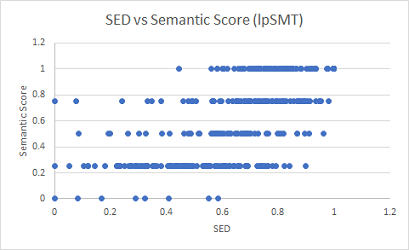
\includegraphics{img/sedvssem_lpSMT.png}
%\label{fig:SedSemlpSMT}
%\end{figure}
%
%\begin{figure}
%\caption{SED vs Semantic (mppSMT)}
%\centering
%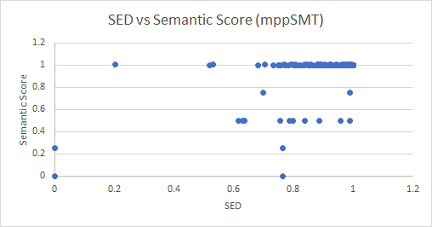
\includegraphics{img/sedvssem_mppSMT.png}
%\label{fig:SedSemMppSMT}
%\end{figure}

%\subsubsection{\textbf{TREED vs Semantic}}
%TREED compares source code at higher level of representation (Syntax Tree). Syntax of source code is the pre-requisite before mentioning about its semantics or functionality. Comparing methods in term of syntax is likely to reflect semantic accuracy better than comparing at lexical level. This argument is proved by our empirical results:

%Technically, a translated method cannot be said to perform any functionality if it cannot be compiled. However, in the Code Migration problem, a translated method which has wrong syntax can still be useful for developers.

%Figure \ref{fig:TREEDmppSMT} shows the scatter plots between 2
%metrics: TREED and Semantic score for the model mppSMT. In general, the result has similar
%trend as in the relation of BLEU and Semantic score: the data points
%are too scattered to show a strong correlation and there are
%several outliers. For a fixed value of Semantic score, TREED score can
%still vary in a large range. However, compared to BLEU, the variation
%is much smaller. For example, a pair of method that has Semantic score
%of 0.5 can possibly have TREED scores in range of 0.7 to 1 while such
%range is 0.5 to 1 for BLEU. TREED shows noticeable improvement over
%BLEU or SED on the correlation with Semantic score on the mppSMT model
%(0.549 to 0.820), on lpSMT model (0.533 to 0.786), and on the GNMT model (0.692 to 0.734).

%\emph{Observation 1:} For a fixed value of Semantic score, there can be many associated TREED values. Specifically, in the model lpSMT, with a Semantic Score of 1, the TREED scores can be varied greatly between 0-1, which was reflected on the top horizontal line of dots in figure \ref{fig:TREEDlpSMT}. Similarly, in the figure \ref{fig:TREEDmppSMT}, with a Semantic Score of 1, the TREED scores are in the range of 0.7 to 1.
%
%\emph{Observation 2:} For a fixed value of TREED, there can be many associated Semantic scores. For example, the figure \ref{fig:TREEDlpSMT} shows that for a high TREED score, for example 0.8, can have Semantic Score from 0.25 to 1. This can be observed by the vertical line of dots in the figure.



% Comparing figure \ref{fig:BleuSemMppSMT} and figure \ref{fig:TREEDmppSMT}, it can be realized that on the model mppSMT, those horizontal lines of dots in figure \ref{fig:BleuSemMppSMT} became shorter in figure \ref{fig:TREEDmppSMT}. It means the variation of TREED score for certain Semantic score is lower. Data points in the figure can also be approximately fitted with a regression line even though there still are some outliers.

%From observation 1, it can be implied that a translated method can have low TREED score, but high Semantic score. On the other hand, from observation 2, a translated method can have high TREED score, but low Semantic score. The two implications above shows that an improvement in TREED is not sufficient nor necessary to improve translation migration quality. However, from observation 3, there is hint of positive improvement that using TREED would reflect Semantic score better than BLEU.

%Issues of TREED that were showed by the figure \ref{fig:TREEDmppSMT} can be explained by two reasons. First, a translated method can be syntactically correct, however still does not have the same functionality as the reference
%code (high TREED score, low Semantic score). Secondly, there
%exists the scenarios of low TREED score with high Semantic score. For
%example, a translated method can have an incorrect place for a
%semicolon, which makes it not compiled. Beside that mistake, if it can
%reflect the functionality of the reference code, it still has a high
%Semantic score. However, due to the increase of coefficient, there is
%an indication that TREED would reflect syntactic correctness better
%than BLEU.

%In certain circumstance, TREED could be used to evaluate SMT-based
%Migration system that focuses on translating correct syntax code.

%\begin{figure}
%\caption{TREED vs Semantic (lpSMT)}
%\centering
%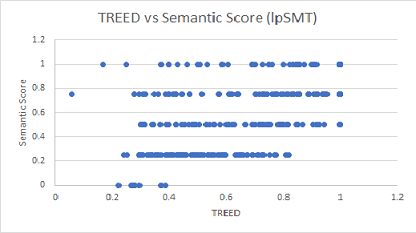
\includegraphics{img/treed_lpSMT.png}
%\label{fig:TREEDlpSMT}
%\end{figure}
%
%\begin{figure}
%\caption{TREED vs Semantic (mppSMT)}
%\centering
%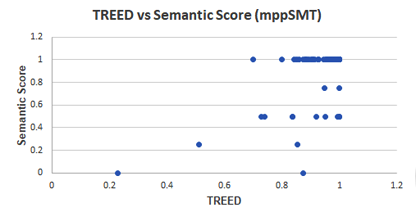
\includegraphics{img/treed_mppSMT.png}
%\label{fig:TREEDmppSMT}
%\end{figure}
%
%\subsubsection{\textbf{GVED vs Semantic}}

%There are studies that compare PDGs to measure the semantic
%similarity. PDGs capture all data and control dependence of program
%elements, and those dependencies are the keys to reflect functionality
%of source code. Therefore, GVED is expected to have the best
%correlation with Semantic score. Our results cement this argument.

%Figure \ref{fig:GVEDmppSMT} shows the scatter plots between 2 metrics:
%GVED and Semantic score when GVED is applicable. There are 240 of such
%points for the model mppSMT in the total of 375 pairs of methods, and
%75 points for lpSMT, respectively. The correlation coefficients between
%GVED and Semantic score are 0.910, 0.823, and 0.927 for the 3 models mppSMT, lpSMT, and GNMT respectively. These values show the better correlations with
%Semantic score than any of the BLEU, SED, and TREED metrics.
%
%significant improvements on both models comparing to any of the other
%3 metrics.
%
%All other three metrics have correlation coefficients with Semantic
%Score less than 0.7 while GVED achieves remarkable correlation
%coefficients of nearly 1.0 .
%
%GVED's promising result makes it an obvious choice to evaluate
%SMT-based Code Migration systems.
%

%A caveat to this is that not all migrated code is sufficiently correct
%to build the corresponding PDGs.
%
%the translated methods have too many errors that cannot be built into
%PDG, or even be compiled.
%That explains the situation in which the number of data points
%available for model lpSMT is too small to draw conclusion about the
%correlation with high confidence. Therefore, even though GVED is a
%metric with highest correlation with Semantic scores, it is not always
%applicable. To cope with its limitation while still utilizing its
%strength in correlation with semantic scores, we explore the
%combination of GVED and other metrics in our novel metric, {\model}.


%\begin{figure}
%\caption{GVED vs Semantic (lpSMT)}
%\centering
%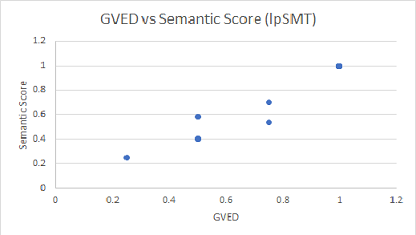
\includegraphics{img/gved_lpSMT.png}
%\label{fig:GVEDlpSMT}
%\end{figure}
%
%\begin{figure}
%\caption{GVED vs Semantic (mppSMT)}
%\centering
%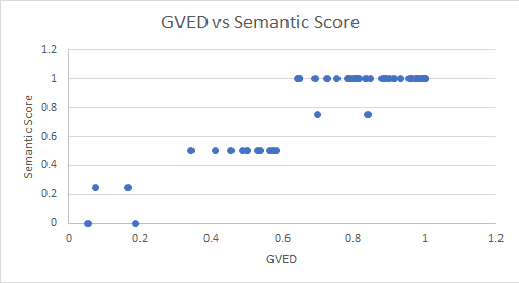
\includegraphics{img/gved_mppSMT.png}
%\label{fig:GVEDmppSMT}
%\end{figure}
